\documentclass[onecolumn, draftclsnofoot,10pt, compsoc]{IEEEtran}
\usepackage{graphicx}
\usepackage{url}
\usepackage{setspace}
\usepackage{cite}
\graphicspath{{./images/}}

\usepackage{geometry}
\geometry{textheight=9.5in, textwidth=7in}

% 1. Fill in these details
\def \CapstoneTeamName{		The Cleverly Named Team}
\def \CapstoneTeamNumber{		58}
\def \GroupMemberOne{			Daniel Grocki}
\def \GroupMemberTwo{			Austin Sanders}
\def \GroupMemberThree{			Owen Loughran}
\def \GroupMemberFour{			David Jansen}
\def \GroupMemberFive{			Brendan Byers}
\def \CapstoneProjectName{		Software product life cycle transformation with Docker container technology}
\def \CapstoneSponsorCompany{	HP}
\def \CapstoneSponsorPerson{		Bryan Crampton}

% 2. Uncomment the appropriate line below so that the document type works
\def \DocType{		%Problem Statement
				%Requirements Document
				%Technology Review
				Design Document
				%Progress Report
				}
			
\newcommand{\NameSigPair}[1]{\par
\makebox[2.75in][r]{#1} \hfil 	\makebox[3.25in]{\makebox[2.25in]{\hrulefill} \hfill		\makebox[.75in]{\hrulefill}}
\par\vspace{-12pt} \textit{\tiny\noindent
\makebox[2.75in]{} \hfil		\makebox[3.25in]{\makebox[2.25in][r]{Signature} \hfill	\makebox[.75in][r]{Date}}}}
% 3. If the document is not to be signed, uncomment the RENEWcommand below
\renewcommand{\NameSigPair}[1]{#1}

%%%%%%%%%%%%%%%%%%%%%%%%%%%%%%%%%%%%%%%
\begin{document}
\begin{titlepage}
    \pagenumbering{gobble}
    \begin{singlespace}
%    	\includegraphics[height=4cm]{coe_v_spot1}
        \hfill 
        % 4. If you have a logo, use this includegraphics command to put it on the coversheet.
        %\includegraphics[height=4cm]{CompanyLogo}   
        \par\vspace{.2in}
        \centering
        \scshape{
            \huge CS Capstone \DocType \par
            {\large\today}\par
            \vspace{.5in}
            \textbf{\Huge\CapstoneProjectName}\par
            \vfill
            {\large Prepared for}\par
            \Huge \CapstoneSponsorCompany\par
            \vspace{5pt}
            {\Large\NameSigPair{\CapstoneSponsorPerson}\par}
            {\large Prepared by }\par
            Group\CapstoneTeamNumber\par
            % 5. comment out the line below this one if you do not wish to name your team
            %\CapstoneTeamName\par 
            \vspace{5pt}
            {\Large
                \NameSigPair{\GroupMemberOne}\par
                \NameSigPair{\GroupMemberTwo}\par
                \NameSigPair{\GroupMemberThree}\par
                \NameSigPair{\GroupMemberFour}\par
                \NameSigPair{\GroupMemberFive}\par
            }
            \vspace{20pt}
        }
        \begin{abstract}
        % 6. Fill in your abstract    
        This document will detail the design of the system we will implement. It will outline the design of the containers and services that will be used in our prototype of HP's PageWide Web Press printers. This document outlines the interaction between our Docker containers as well as how Kubernetes will manage them. The current system design is also described here since our prototype must work with the existing system and workflow.
        
        \end{abstract}     
    \end{singlespace}
\end{titlepage}
\newpage
\pagenumbering{arabic}
% 7. uncomment this (if applicable). Consider adding a page break.
%\listoffigures
%\listoftables
\clearpage

% 8. now you write!


\section{Introduction}

\subsection{Scope}

The software outlined in this document is meant to repackage the current software on the servers that control HP’s industrial sized printers. Our goal is reduce down time for when printers are updated through constant integration, and reduce the amount of hardware needed by fitting more than one microservice on each server.


\subsection{Purpose}

The purpose of this Software Specification Document is to provide an overview for how the project Software Product Life Cycle Transformation With Docker Container Technology will be designed and executed. To accomplish this, the document will outline our system architecture and functionalities.


\subsection{Intended Audience}

This document is intended for the Sponsors of the Capstone project and the Capstone Instructors. This document is to serve as a guide for the development team to accomplish the project in a way that is agreed upon with the sponsors.


\subsection{Definitions}
\begin{itemize}
    \item \textbf{Docker:} Open source software platform to create, deploy and manage virtualized application containers on a common operating system\cite{tech}.
    
\item \textbf{Application Containerization:} OS-level virtualization method used to deploy and run distributed applications without launching an entire virtual machine\cite{tech}.

\item \textbf{Docker Image:} A file, comprised of multiple layers, used to execute code in a Docker container\cite{tech}.

\item \textbf{Docker Hub:} Similar to GitHub, Docker Hub is a cloud based registry service that allows you to link code repositories, build images and test them.
    
\item \textbf{Kubernetes:} Open source system used to manage Linux containers across private, public and hybrid cloud environments\cite{tech}.



\item \textbf{Kubernetes Pod:} Smallest deployable computing units in the open source Kubernetes container scheduling and orchestration environment\cite{tech}.

\item \textbf{Server Operating System:} an operating system specifically designed to run on servers, which are specialized computers that operate within a client/server architecture to serve the requests of client computers on the network\cite{tech}.

\item \textbf{Linux Server:} Linux-based server operating system\cite{tech}.

\item \textbf{Windows:} A group of operating systems created and maintained by Microsoft

\item \textbf{Riak:} A distributed key valued database.

\item \textbf{Beanstalk:} An open source product that manages job request queues.

\item \textbf{Jenkins:} Jenkins is an automation server that integrates with source controls to automatically build, test and deploy code.

\item \textbf{Artifactory:} A binary repository management software. It centralizes the projects binaries, so developers all have access to the same tools.

\item \textbf{Websocket:} Instead of streaming data, websockets are built on a message based transport system that is bi-directional.
Both the client and server can communicate to each other at the same time with low latency.
Data is packaged into messages and is reassembled once it arrives at it's destination.

\item \textbf{HTTP:} HyperText Transfer Protocol is a request-response protocol in a client server computing model. It is one method used for processes to interact with each other.


\item \textbf{API:} An API (Application Program Interface) is a set of endpoints used to interact with a software.

\item \textbf{Groovy:} An object oriented programming language built around the Java platform. It can be used as both a scripting language and programming language.

\item \textbf{Gradle:} Gradle is an open source build automation tool. Designed for use with the Groovy language.

\item \textbf{Printing Press:} Printing press is a large machine used to print images and text at high volume.



\end{itemize}

\section{System Overview}

The Software Product Life Cycle Transformation With Docker Container Technology is a software aimed at reformatting how HP’s industrial printers' servers. Currently, the servers do not optimize the hardware on board, and when a service has to be updated or changed the entire system has to come offline. On occasion HP even has to send an engineer to the physical location to fix the machine. The aim of this project is to alleviate some, if not all, of these issues.

To decrease the downtime of servers while being updated the project will use a combination of Docker and Kubernetes to ‘containerize’ the entire micro service on the servers themselves. When properly packaged into images the server should suffer no downtime as a result. This is because images can be removed and updated remotely, and while the micro service is running. Then when Kubernetes or another container requests a new instance of that image it can pull the new updated image all while the system is running. The container will retain the same functionality, just with improved performance.

The second problem that will be addressed in this project is the inefficient use of the server's hardware. Currently with the micro service running outside of containers it is difficult to run more than one micro service without interfering with each other. With the use of Kubernetes it would be possible to encapsulate each individual micro service into their own pods. This way the system could dictate the amount of resources allocated to them. With this technology in place it would become possible to run more than one instance of each micro service on each individual server. That means the printer would be able to run on a server with fewer instances of Linux and Windows.

Overall the goal of the project ‘Software Product Life Cycle Transformation With Docker Container Technology’ is to reduce the downtime of the printers, and reduce the amount of hardware required to run the micro service as a whole.




\newpage
\section{Architecture}

\subsection{System Architecture}

The system will implement a way for developers to easily develop code and create working images. The dependencies for the developer’s code will come from Artifactory. We will be using Git and Github to implement version control. Jenkins will allow for continuous integration with the code pushed to Github. When code is pushed, Jenkins will build and test the code and pull in all the Artifactory dependencies. If this succeeds, we then can take the built image from Jenkins and put it in our image repository. The image repository for this project is Docker Hub. This will contain all the images that we create for this project. In the grand scheme of things, these images will then be able to be pulled by the test teams to test, and the DevOps team to deploy to production. The images on the repository are the images that Kubernetes will be managing. 

It is important to consider how our project will integrate with the current workflow at HP. Since our project needs to work in their current system, we need to consider the current system in our design process to make sure we are designing our system in a way that works.

\begin{figure}[h]
    \centering
    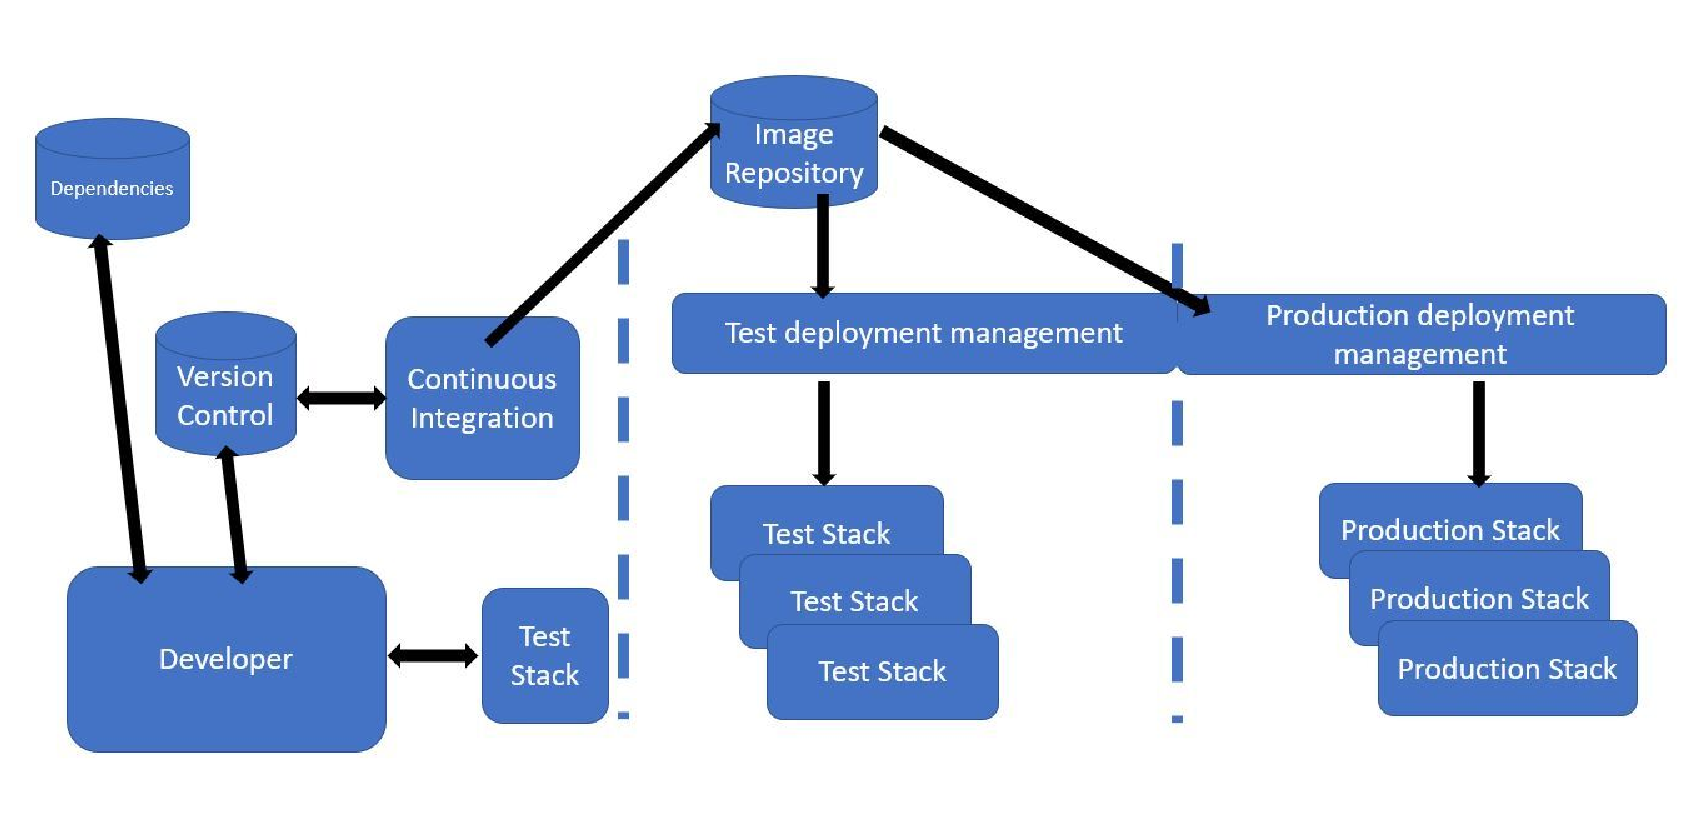
\includegraphics[width=\textwidth, height=8cm]{prjct_arch.eps}
    \caption{This illustrates the workflow we should expect our prototype to experience, when implement it in the current system.}
\end{figure}

\subsection{Container Design}

The Linux servers will run containers that will communicate to parse a PDF and prepare it for printing. There are 5 different containers that we will need: Beanstalk, Riak, WorkManager, WorkerA, and WorkerB. Riak and Beanstalk are open source projects, but we will need to write Groovy code and containerize WorkManager, WorkerA, and WorkerB. The parsing and creation of the PDF will be accomplished by the combined work of these processes. 
\newpage

\begin{figure}[h]
    \centering
    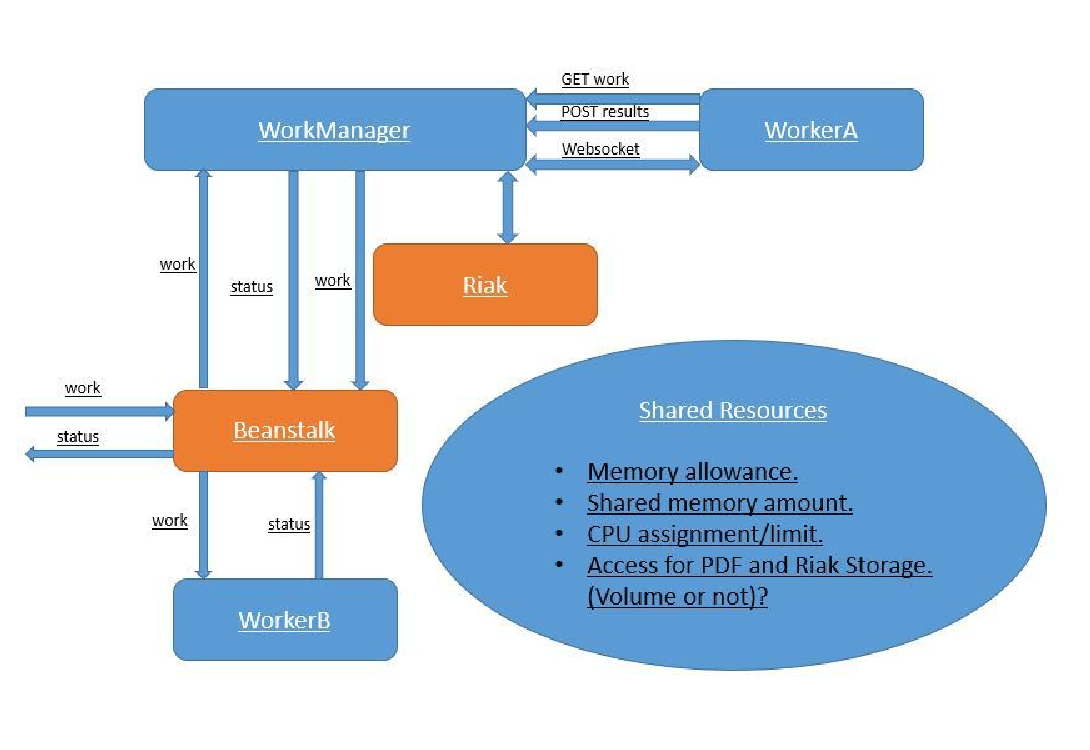
\includegraphics{prjct_arch_workers.eps}
    \caption{The 5 containers will interact with each other in this way. All these containers should share a set amount of resources on the server}
\end{figure}


\begin{itemize}
    \item Beanstalk
    
    Beanstalk is an open source product that is used for queuing up the requests. Since it is open source, there is already existing images for it published and we can build off of that. It is used to queue up requests for the system. These requests can either be new work from the outside or work going from the WorkManager to WorkerB.

    \item Riak
    
    Riak is also an open source project that has already been containerized. Riak will be used to store the final result of the work. After WorkerA and WorkerB have successfully completed their steps, the complete project will be stored in Riak.
    
    \item WorkManager
    
    The WorkManager is the one in charge om managing the Workers. It receives work requests from Beanstalk. It also receives GET and POST requests from WorkerA. It will use a websocket to communicate with WorkerA. The WorkManager will also be responsible for communicating with Riak to store and fetch information. 
    
    \item WorkerA
    
    WorkerA is responsible for inserting content into the PDF that we are trying to print. It will make use of the PDFBox library to do this. 
    It will receive work via a web socket from the work manager and save its results to shared memory with WorkerB. 
    WorkerA sends back a success or failure result to the WorkManager based whether it was able to successfully add content. 
    
    \item WorkerB
    
    When the WorkManager has received a success from WorkerA, it will then queue up a request via Beanstalk for WorkerB. WorkerB is then responsible for the imposition of the PDF pages. This means that it must process the work from WorkerA. WorkerB will access the memory it shares with WorkerA to receive WorkerA’s results. It will then process the work using the PDFBox library and then update the status of the work once it is done. This status is sent back to Beanstalk.
    
    
\end{itemize}

There will be a single WorkManager, but multiple of each Worker A and Worker B as shown in the next picture. All of these Worker A’s and B’s will communicate with the same WorkManager. Once all of these images have been deployed onto a server, we will use Kubernetes to combine them into a pod that only communicates with itself. By doing this, we open up the possibility to running multiple sets of these pods on a single server. Each of these pods will be allocated a certain amount of resources that all the services running in it will have to share. These resources include memory, Riak Storage access, and CPU usage. These pods should not overlap and Workers on one pod should not know about or communicate with a WorkManager on another pod. 

\begin{figure}[h]
    \centering
    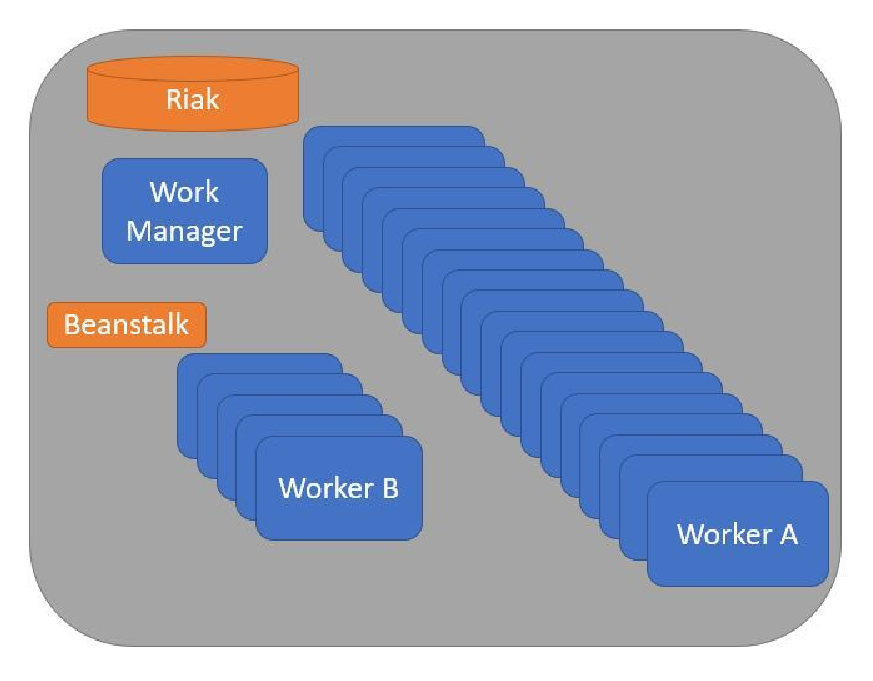
\includegraphics{prjct_arch_pod.eps}
    \caption{There will be multiple instances of WorkerA and WorkerB running in a pod. All of this is considered one pod and must share the same resources and shouldn't interact with any other pod}
\end{figure}

\subsection{Design Reasoning}
The system architecture is designed this way mainly to model the existing system. Since everything we are working with is already in production, we must make sure to match the current workflow. We must design our system to fit into their current process of creating updates, testing, and deploying. The fundamental architecture of the Workers must stay the same since we are not changing how they do the PDF parsing. Our goal is to containerize the services to decreases resource consumption. By maintaining the architecture they have for the communication between the 5 different containers, our prototype will be the most accurate and the most useful to HP.

\section{Perspective}
In order to satisfy HP our solution needs to be efficient, the main goal with the containerization is to reduce the amount of resources they need to use in order to process print jobs on their printing presses. The perspective section will expand upon the viewpoints we took when designing our solution and choosing technologies in order to achieve this implementation: Context, Composition, Logic, Structure, and Interaction.

\subsection{Context Viewpoint}
The context of the project we are creating for HP is essential to the decisions we made. This solution is meant purely to increase HP’s DevOps efficiency and decrease the server costs of supporting their printing presses. The tools we implement will be used by software engineers to deploy and manage their software, and as such flexibility and power will be prioritized over ease of use and simplicity.
\subsection{Composition Viewpoint}
The composition of our project is built up of many different components that must communicate with each other in order to form a single process. Within our design we have decided to containerize each individual component, these containers will then communicate with one another. It is very important that each component will be capable of sending and receiving data from it's container. This data must also be sent to and received from the correct components within the process. Once each component has achieved this the entire process will then be containerized. 
\subsection{Logic Viewpoint}
The logic behind the design is that it will increase utilization of valuable server resources, it will also allow for less downtime associated with updates and changes to a process. When each component of a process is containerized it allows for individual pieces to be updated without needing to update the entire process. This done by simply swapping an old container out with a new updated container. When each process is put in to a container it will allow multiple processes to run on a single server without interfering with one another. 
\subsection{Structure Viewpoint}
The structure of our design will require two layers of containers, one layer is a group of containers, the other layer will encapsulate that group of containers. In the first layer each component of a process will be stored in an independent container from the other components within the process. Inside these containers will be each component and all of the necessary dependencies for it. In the next layer there will be a container for the entire process. This structure will allow for separate processes to run on a single server, it also makes updates and changes to each process much simpler.
\subsection{Interaction Viewpoint}
Our design makes it possible for multiple duplicate processes to run on a single server without them interfering with one another. Each individual process is comprised of many different components. Each component in a process is designed to interact with other components within the process in a certain way. It is also important in our design to ensure that components within one process are not communicating with components in other processes on the server. 


\section{Component Design}

\subsection{Docker}
\subsubsection{Structural Element}
Each component within the printing process will be containerized using Docker containerization technology. The components that will make up the process are all explained in section 3.2. Within each container we will be storing both the component itself and any dependencies that it needs in order to function properly. Each container will also be responsible for communicating with other containers within the process. This means each container must be capable of both sending and receiving data. 
\subsubsection{Design Rationale}
The rationale behind the use of Docker as one of the components within the project is that containerization offers many benefits. One of the main benefits is that containerization can significantly reduce downtime of a process. When a single component needs to be updated or changed Docker allows you to create a new updated container and swap it out with the current corresponding container in the process. This means the entire process will not experience downtime when updating individual components, and any downtime from swapping out a container will be minimal \cite{docker}. 

\subsection{Kubernetes}
\subsubsection{Structural Element}
Kubernetes is a component that will be used in our project in order to manage our containers. Specifically we will be looking in to Kubernetes pods in order to encapsulate our entire printing process. Each pod will represent an actual running printing process on the server. These pods will allow us to easily manage our containers as a single entity, it also allows sharing of resources within the pod \cite{kub}. 
\subsubsection{Design Rationale}
The rationale behind the use of Kubernetes is that it will allow us to run multiple duplicate processes on a single server without them interfering with one another. Currently the issue with the non containerized processes is that if you run multiple processes on a single server they may communicate with the wrong process components. This is because the components within the processes are identical to each other, each process will still be responsible for performing a different job though. This means if there is interference from one process to another they likely will not properly complete their job. With Kubernetes we are able to encapsulate each process in to pods. These pods will then perform each process completely independently of one another and there will be no interference's between them. 

\subsection{Jenkins}
\subsubsection{UI Element}
Jenkins offers a UI element that makes the creation of continuous integration easy. Within this UI we are capable of connecting our Jenkins build systems to different branches of our GitHub. It also allows us to pipeline the containers that are successfully built on Jenkins to our Docker Hub account where the containers will be stored. 
\subsubsection{Structural Element}
Jenkins will mainly be used for unit testing of our containers. When each container is built we will need to test that it is functioning properly using unit tests. These tests will depend on what the purpose of the container is. Jenkins offers us a way to run these tests every time that new code is pushed to our GitHub branches. When code is pushed Jenkins will run the tests we have setup and notify us if they failed or succeeded. If tests are successful the newly built containers will be sent to our Docker Hub account.
\subsubsection{Design Rationale}
The design rationale behind the use of Jenkins for continuous integration is quite simple, it allows us to know that we are properly creating functioning containers. Jenkins will allow for significantly less debugging time because it will notify us if our tests have passed or not, every single time new code is pushed to GitHub. This means we will have more time to work on completing the project and spend less time debugging code. It will also make it so our Docker Hub does not get filled with junk containers that don't function properly since the container won't be added unless they passed all tests.
\bibliographystyle{ieeetr}
\bibliography{references}

\end{document}
